\subsubsection{CIFAR-10 and t-SNE Interpretation}\label{sec:cifar-10-and-t-sne-interpretation}

Until now, we argued theoretically that:
\begin{itemize}
    \item Images are represented as very high-dimensional vectors;
    \item k-NN compares images using pixel distances;
    \item Pixel distances do \textbf{not} correspond to semantic similarity, i.e., perceptual distances.
\end{itemize}
Now, we ask ourselves: \emph{\textbf{can we actually see this phenomenon in practice?}} The answer is \textbf{yes}, using \textbf{t-SNE}.

\highspace
Recall that each CIFAR-10 image is represented as $x \in \mathbb{R}^{3072}$. Obviously, we cannot visualize points in a 3072-dimensional space. The idea is therefore: project the 3072-dimensional vectors into \textbf{2 dimensions}, while trying to preserve their neighbourhood relationships. This is exactly what \textbf{t-SNE} does.

\highspace
\begin{flushleft}
    \textcolor{Green3}{\faIcon{question-circle} \textbf{What is t-SNE?}}
\end{flushleft}
\definition{t-distributed Stochastic Neighbor Embedding (t-SNE)} is a \textbf{dimensionality reduction technique} that is particularly well-suited for the visualization of high-dimensional datasets. We don't go into the details of how t-SNE works because we will use it only as a \textbf{visualization tool}.

\highspace
Its goal is simple: \hl{given a set of high-dimensional vectors, t-SNE finds a low-dimensional representation of the data that preserves neighbourhoods.} For example, if two images are close in the original space, they should also appear close in the 2D visualization. Likewise, if two images are far apart, they should also appear separated.

\highspace
\begin{flushleft}
    \textcolor{Green3}{\faIcon{question-circle} \textbf{What can we expect to see?}}
\end{flushleft}
Imagine Euclidean distance perfectly reflected semantic similarity. Then, all images of the same class would be clustered together in the 2D visualization. But this is exactly what we would hope for if pixel distances were approximately equal to perceptual distances. In other words, if pixel distances were a good proxy for semantic similarity, we would expect to see \textbf{well-separated clusters of images of the same class} in the t-SNE visualization.

\highspace
\textcolor{Green3}{\faIcon{question-circle} \textbf{What actually happens on CIFAR-10?}} As we will see, \textbf{this is not what happens}. Instead, the classes are heavily mixed. The \hl{different classes overlap significantly.} This means that, in the original pixel space:
\begin{itemize}
    \item Many dogs are closer to cars than to other dogs;
    \item Many airplanes are close to birds;
    \item Many ships are mixed with trucks.
\end{itemize}
The neighbourhoods are \textbf{not semantic}. And we have already argued the reason: the Euclidean distance only measures pixel-wise differences independently of the spatial structure of the image. Thus, two images with similar backgrounds or colours may therefore be close in pixel space even if they depict completely different objects.

\highspace
\begin{figure}[!htp]
    \centering
    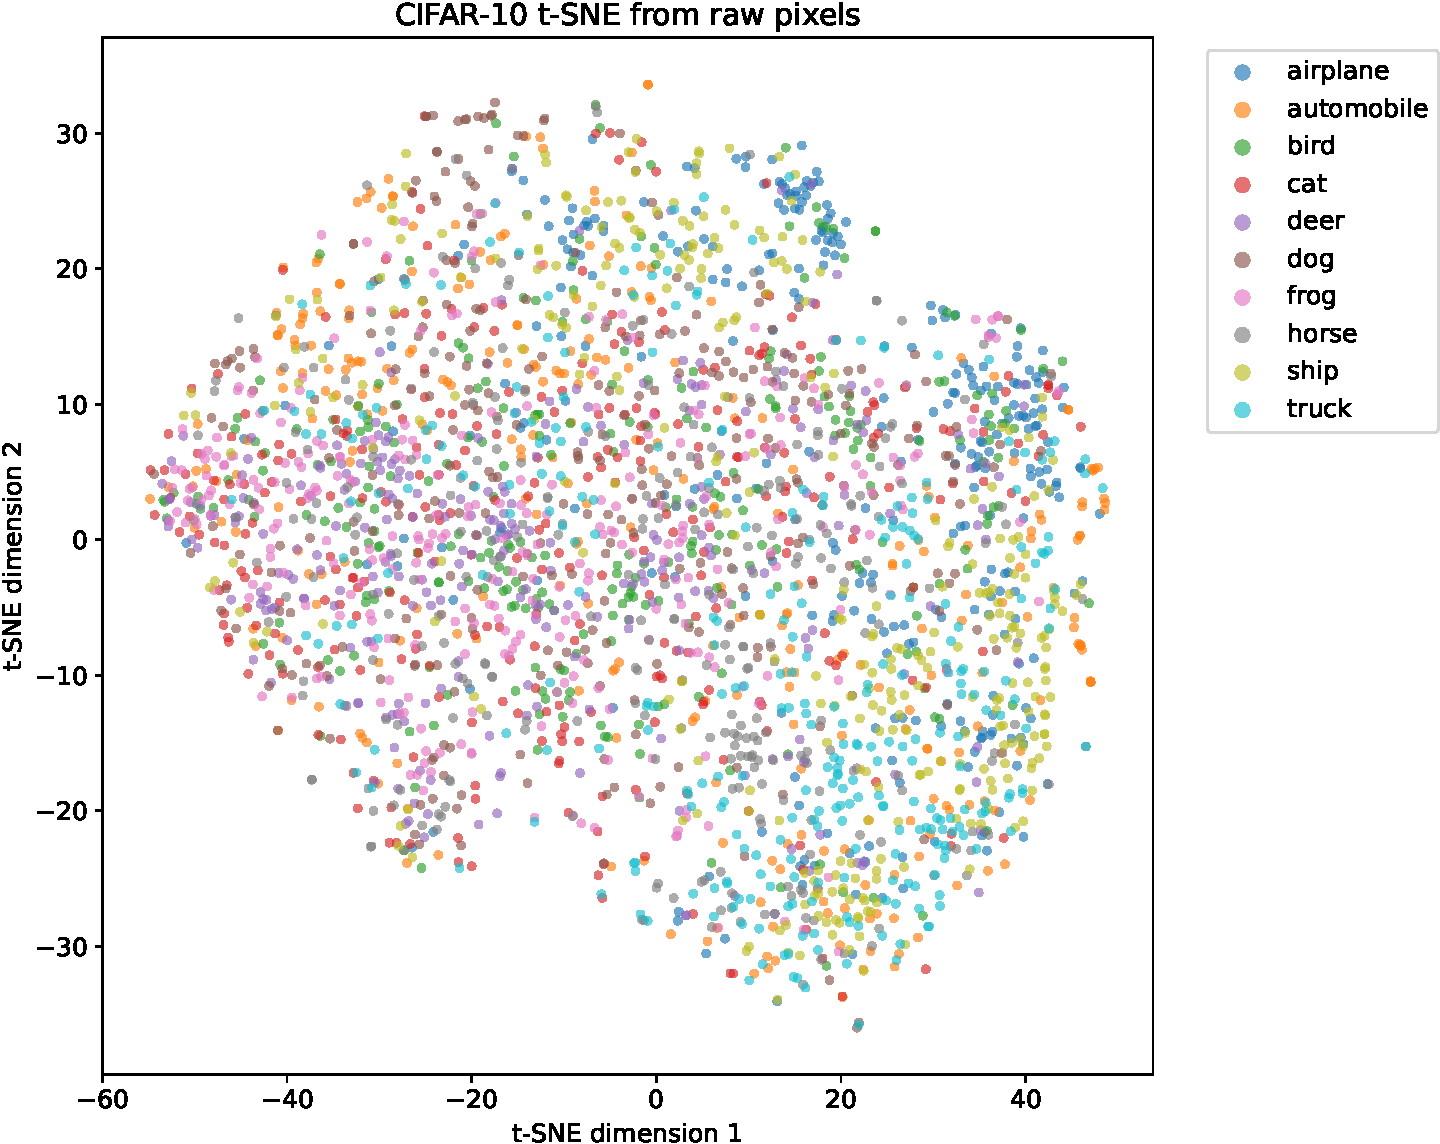
\includegraphics[width=\textwidth]{img/cnn/cifar10-raw-pixels-tsne.pdf}
    \captionsetup{singlelinecheck=off}
    \caption[]{t-SNE visualization of CIFAR-10 images in the original pixel space.}
    \label{fig:cifar10-raw-pixels-tsne}
\end{figure}

\noindent
Each image is composed of $32 \times 32$ pixels, each with three RGB values. The t-SNE algorithm projects the $3072$-dimensional vectors into 2D while trying to preserve neighbourhoods. The points are colored according to their class.

\highspace
\textcolor{Green3}{\faIcon[regular]{lightbulb} \textbf{Observation.}} Every color is mixed with every other color. There are \textbf{no clear clusters} and almost every class overlaps with the others. For example airplanes are mixed with trucks, ships are mixed with automobiles, and so on. There are only tiny local groups. This \hl{phenomenon occurs because each image is represented by $3072$ RGB values.} Two images that are semantically identical can have very different pixel values.

\highspace
Note: we are \hl{not applying any k-NN classifiers here.} We have found that when images are compared using pixel distances, as the k-NN algorithm does, many images of different classes appear closer to each other than to images of the same class. This is precisely why k-NN performs poorly on CIFAR-10.

\newpage

\begin{figure}[!htp]
    \centering
    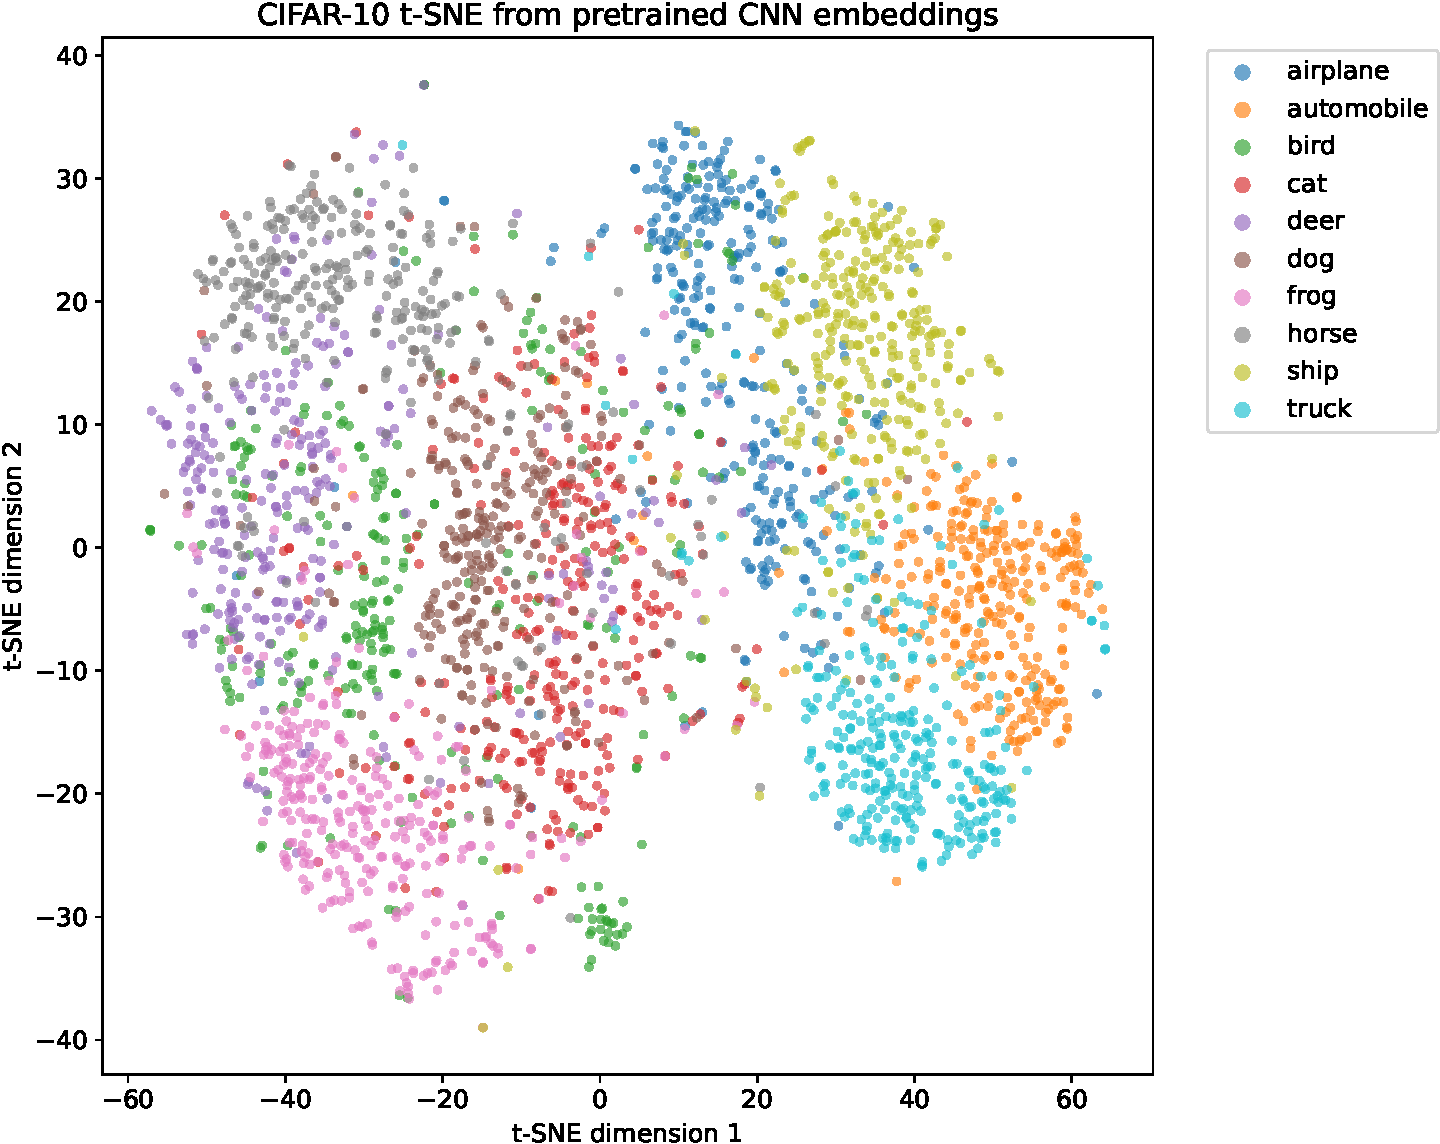
\includegraphics[width=\textwidth]{img/cnn/cifar10-cnn-embeddings-tsne.pdf}
    \captionsetup{singlelinecheck=off}
    \caption[]{t-SNE visualization of CIFAR-10 images in the CNN embedding space.}
    \label{fig:cifar10-cnn-embeddings-tsne}
\end{figure}

\noindent
Each image is passed through a Convolutional Neural Network (CNN), specifically a pretrained ResNet18. The final classification layer is removed, and the output of the feature-extraction part of the network is used as a new vector representation of the image. Therefore, each image is represented by a $512$-dimensional embedding.

\highspace
The t-SNE algorithm projects these $512$-dimensional vectors into two dimensions while trying to preserve local neighbourhood relationships. Each point represents one image and is coloured according to its ground-truth class.

\highspace
\textcolor{Green3}{\faIcon[regular]{lightbulb} \textbf{Observation.}}
The \hl{CNN produces a representation that is much more semantically meaningful than the original pixel representation.} Images belonging to the same class tend to be close to one another, while different classes form more distinguishable regions. For example, airplanes, ships, automobiles, and trucks are much more clearly separated than in the raw-pixel representation.

\highspace
However, the classes are not perfectly separated. Some semantically related categories, especially animals such as cats, dogs, deer, and horses, still partially overlap because they share visual features such as fur, heads, eyes, legs, and similar body shapes.

\highspace
Since neighbourhoods in this embedding space are more semantically meaningful, a k-NN classifier applied to these embeddings would be expected to perform much better than a k-NN classifier applied directly to raw pixels.

\highspace
This is also the idea behind \hl{\textbf{image retrieval systems}}, where a query image and the images in a database are converted into embeddings and compared in the learned feature space rather than in the original pixel space.

\highspace
\hl{This experiment motivates the use of Convolutional Neural Networks (CNNs) for image classification.} Using any pixel-wise distance measure, and in particular the Euclidean distance, is \textbf{not sufficient to capture semantic similarity} (see \autoref{fig:cifar10-raw-pixels-tsne}). Instead, a \textbf{CNN learns an embedding (latent representation)} in which semantically similar images are close together (see \autoref{fig:cifar10-cnn-embeddings-tsne}).